\chapter{Конструкторская часть}

В данном разделе предсатвлены требования к программному обеспе-
чению, а также схемы алгоритмов, выбранных для решения поставленной
задачи.

\section{Требования к программному обеспечению}
Программа должна предоставлять доступ к функционалу:
\begin{itemize}
	\item задать положение камеры и направление взгляда;
	\item изменение положения источника света;
	\item конфигурация облачного неба с помощью загрузки погодной карты;
	\item варьирование параметров облаков;
\end{itemize}

К программе предъявляются следующие требования:
\begin{itemize}
	\item время отклика программы должно быть менее 50 мс;
	\item программа должна корректно реагировать на любые действия пользователя;
\end{itemize}

\section{Алгоритм визуализации}

Попадая в облачный объем необходимо сделать $ N $ шагов, на каждом из которых вычисляется плотность в точке пространства и ее освещенность, используя эти данные итеративно вычисляется значение цвета пикселя. 

\begin{figure}[h]
	\centering
	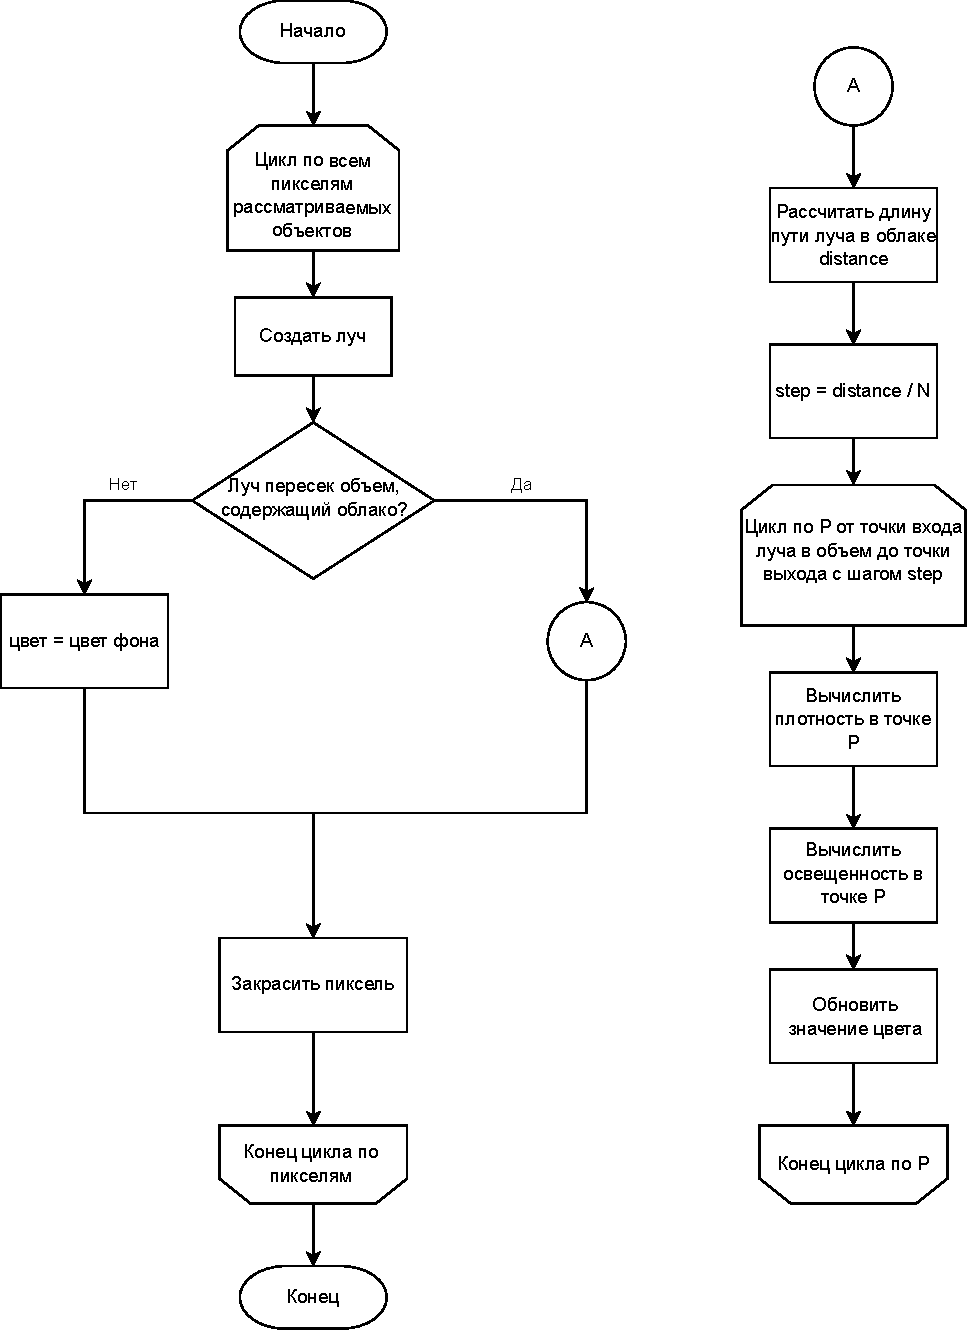
\includegraphics[width=0.9\textwidth]{assets/img/renderscheme.pdf} % замените на имя вашего файла
	\caption{Схема визуализации облаков с помощью алгоритма Ray Marching}
	\label{fig:renderscheme}
\end{figure}

